% =============================================================
% STANDALONE DRAFT OF CHAPTERS 2 AND 3
% Compile on its own (pdflatex -> bibtex -> pdflatex x2).
% When merging back into main.tex: delete the filecontents block
% below and the preamble, and keep only the material between the
% two markers "BEGIN BODY" and "END BODY".
% =============================================================

% --- PLACEHOLDER BIBLIOGRAPHY -------------------------------
% These entries exist only so that this file compiles on its own.
% They are NOT verified. Replace with the real biblio.bib on merge.
\begin{filecontents*}{biblio_ch23.bib}
@article{Long_Lag2025,
  author = {De Graeve, Ferre and Westermark, Andreas},
  title = {The Long and the Short of It: Inference on Structural Parameters from Long-Lag VARs},
  journal = {Working paper},
  year = {2025}}
@article{Baumeister2025,
  author = {Baumeister, Christiane},
  title = {Placeholder title},
  journal = {Working paper},
  year = {2025}}
@article{Ravenna2007,
  author = {Ravenna, Federico},
  title = {Vector Autoregressions and Reduced Form Representations of {DSGE} Models},
  journal = {Journal of Monetary Economics},
  volume = {54},
  pages = {2048--2064},
  year = {2007}}
@techreport{ACEL2005WP,
  author = {Altig, David and Christiano, Lawrence J. and Eichenbaum, Martin and Lind{\'e}, Jesper},
  title = {Firm-Specific Capital, Nominal Rigidities and the Business Cycle},
  institution = {NBER Working Paper 11034},
  year = {2005}}
@article{ACEL2011,
  author = {Altig, David and Christiano, Lawrence J. and Eichenbaum, Martin and Lind{\'e}, Jesper},
  title = {Firm-Specific Capital, Nominal Rigidities and the Business Cycle},
  journal = {Review of Economic Dynamics},
  volume = {14},
  pages = {225--247},
  year = {2011}}
@article{CEE2005,
  author = {Christiano, Lawrence J. and Eichenbaum, Martin and Evans, Charles L.},
  title = {Nominal Rigidities and the Dynamic Effects of a Shock to Monetary Policy},
  journal = {Journal of Political Economy},
  volume = {113},
  pages = {1--45},
  year = {2005}}
@article{CEV2006,
  author = {Christiano, Lawrence J. and Eichenbaum, Martin and Vigfusson, Robert},
  title = {Assessing Structural {VAR}s},
  journal = {NBER Macroeconomics Annual},
  year = {2006}}
@article{ChariKehoeMcGrattan2008,
  author = {Chari, V. V. and Kehoe, Patrick J. and McGrattan, Ellen R.},
  title = {Are Structural {VAR}s with Long-Run Restrictions Useful in Developing Business Cycle Theory?},
  journal = {Journal of Monetary Economics},
  volume = {55},
  pages = {1337--1352},
  year = {2008}}
@article{FVRRS2005,
  author = {Fern{\'a}ndez-Villaverde, Jes{\'u}s and Rubio-Ram{\'i}rez, Juan F. and Sargent, Thomas J. and Watson, Mark W.},
  title = {{ABC}s (and {D}s) of Understanding {VAR}s},
  journal = {American Economic Review},
  volume = {97},
  pages = {1021--1026},
  year = {2007}}
@article{Forni_Gambetti_Sala2016,
  author = {Forni, Mario and Gambetti, Luca and Sala, Luca},
  title = {Placeholder title},
  journal = {Working paper},
  year = {2016}}
@article{Humble_VARs_2026,
  author = {Placeholder, A.},
  title = {Humble {VAR}s},
  journal = {Working paper},
  year = {2026}}
@article{Jorda2024long_run_mp,
  author = {Jord{\`a}, {\`O}scar and Kozicki, Sharon},
  title = {Placeholder title},
  journal = {Working paper},
  year = {2024}}
@article{Plagborg-Moller_Wolf2021,
  author = {Plagborg-M{\o}ller, Mikkel and Wolf, Christian K.},
  title = {Local Projections and {VAR}s Estimate the Same Impulse Responses},
  journal = {Econometrica},
  volume = {89},
  pages = {955--980},
  year = {2021}}
@article{Ludwig2026,
  author = {Ludwig, Placeholder},
  title = {Placeholder title},
  journal = {Working paper},
  year = {2026}}
@article{Hall_Inoue_Nason_Rossi2012,
  author = {Hall, Alastair R. and Inoue, Atsushi and Nason, James M. and Rossi, Barbara},
  title = {Information Criteria for Impulse Response Function Matching Estimation of {DSGE} Models},
  journal = {Journal of Econometrics},
  volume = {170},
  pages = {499--518},
  year = {2012}}
@article{SM2007,
  author = {Smets, Frank and Wouters, Rafael},
  title = {Shocks and Frictions in {US} Business Cycles},
  journal = {American Economic Review},
  volume = {97},
  pages = {586--606},
  year = {2007}}
\end{filecontents*}

\documentclass[12pt, a4paper]{article}
\usepackage[margin=1in]{geometry}
\usepackage[english]{babel}
\usepackage[utf8]{inputenc}
\usepackage{setspace}
\onehalfspacing
\usepackage{amsmath}
\usepackage{amssymb}
\usepackage{bm}
\usepackage{microtype}
\usepackage{graphicx}
\usepackage{booktabs}
\usepackage{placeins}
\usepackage{xcolor}
\definecolor{PadovaRed}{HTML}{B20E10}
\long\def\tbd#1{{\color{PadovaRed}\textbf{[TBD:} #1\textbf{]}}}
\usepackage{natbib}
\usepackage[colorlinks=true, citecolor=PadovaRed, linkcolor=black, urlcolor=black]{hyperref}

\setcounter{section}{1}

\begin{document}

\begin{center}
{\large\textbf{Chapters 2 and 3, standalone working draft}}\\[2pt]
{\small Restructured skeleton. Prose is provisional, citations are placeholders.}
\end{center}
\vspace{0.5cm}

% =============================================================
% BEGIN BODY
% =============================================================

% =============================================================
% 2. TRUNCATION BIAS
% =============================================================
\section{Truncation Bias and the Case for Long-Lag VARs}
\label{sec:truncation}

A VAR used for structural inference is exposed to several distinct biases: small sample bias,
identification bias \citep{Forni_Gambetti_Sala2016}, and truncation bias \citep{Long_Lag2025,
Ravenna2007, ChariKehoeMcGrattan2008}. This chapter is about the third, and about the way it
contaminates the second.

The argument runs in three steps. First, the condition usually invoked to licence a VAR, that
the model admits an exact infinite order VAR representation, is not the condition the present
exercise needs, and abandoning it does not weaken the case for care over the lag order but
strengthens it. Second, truncation distorts the estimated responses at every horizon, and it
does so in two distinct ways depending on whether the horizon lies inside or outside the
estimated lag structure. Third, and as a consequence, the lag order is not a nuisance setting
to be delegated to an information criterion. It should be chosen to be consistent with the
horizons that the research question, and in impulse response matching the estimator itself,
actually use.

\subsection{What the VAR is required to deliver}
\label{sec:whatrequired}

The textbook justification for confronting a DSGE model with a VAR runs through a chain of
conditions. The log-linearised solution is written in state space form; if the system is
square, so that the number of structural shocks equals the number of observables, and if the
Poor Man's Invertibility Condition of \citet{FVRRS2005} holds, then the state space system can
be inverted into a VAR($\infty$) in the observables; the researcher then truncates that
representation at some finite $p$. On this reading the VAR is the exact reduced form of the
model, and truncation is the only approximation being made.

The chain is a sufficient condition for a particular and rather strong interpretation of the
VAR. It is not a necessary condition for the VAR to be useful. Impulse response matching makes
a weaker claim. The statement is not ``my model generated the data'' but ``whatever generated
the data, the response of these variables to this shock looks like this over these horizons,
and my model should reproduce it''. \citet{Forni_Gambetti_Sala2016} make the point directly:
fundamentalness is ``extremely and unnecessarily restrictive'', because ``in several cases
fundamentalness is not needed. The researcher is often interested in assessing the transmission
mechanisms of a single shock.'' What matters ``is not whether we have fundamentalness or not,
but whether we have enough information to get a reasonably good approximation for the specific
shocks of interest''.

This reframing is liberating, but it should not be misread. Once the VAR is no longer defended
as the exact representation of anything, its entire claim on our attention is that it
approximates the responses of interest well over the horizons of interest. Truncation is
precisely what governs the quality of that approximation. Dropping the VAR($\infty$)
requirement therefore does not make the lag order a free parameter. It concentrates the whole
burden of the exercise onto it.

\subsection{A simple illustration}

Following \citet{Long_Lag2025}, consider a data generating process in which $y_t$ depends on
two exogenous variables,
\begin{equation}
    y_t = x_{1t}\beta_1 + x_{2t}\beta_2 + \epsilon_t .
\end{equation}
Estimating the relationship while omitting $x_{2t}$,
\begin{equation}
    y_t = x_{1t} b_1 + e_t ,
\end{equation}
delivers a biased coefficient unless the regressors are orthogonal,
$\mathbb{E}(b_1)\neq\beta_1$, and an upward biased residual variance, $s^2 > \sigma^2$. Both
distortions matter in what follows, and the second is the one usually forgotten.

The same logic carries over to a VAR. Let
\begin{equation}
    Y_t = B_1 Y_{t-1} + \dots + B_p Y_{t-p} + u_t,
    \qquad \mathbb{E}[u_t u_t'] = \Sigma_u ,
    \label{eq:var}
\end{equation}
with $p \ll p^{*}$, where $p^{*}$ denotes the true lag order. Omitting lags $p+1$ onwards
biases the retained coefficients, because in any persistent system the omitted regressors are
correlated with the retained ones, and inflates $\Sigma_u$, because variation that belongs to
the systematic part of the process is pushed into the residual. Since the structural impulse
responses are a function of both objects,
\begin{equation}
    \mathrm{IRF} = f\bigl(B(L), \Sigma_u\bigr),
    \label{eq:irf_f}
\end{equation}
they inherit both distortions. Note that this already implies something the horizon
discussion below will sharpen: because $\Sigma_u$ enters the identification, even the impact
response at $h=0$ is affected by lags the researcher chose not to include.

\subsection{Two channels: pure truncation and identification bias}

\citet{Ravenna2007} separates the distortion into two channels. The first is \emph{pure
truncation bias}: a VAR($p$) sets all coefficients beyond lag $p$ to zero and therefore does
not describe the true dynamics. The second is \emph{identification bias}: where the
autoregressive coefficients enter the matrix mapping reduced form innovations into structural
shocks, truncation corrupts that mapping as well. The identification bias arises \emph{even
when the identifying assumptions are correct}, and both results are established in population,
so neither is an artefact of small samples.

Two implications matter here. First, \citet{Ravenna2007} finds the identification channel to be
the dominant one. Second, and more useful for the empirical work, the two channels do not treat
all identification schemes alike. A short-run recursive scheme recovers the structural impact
matrix from $\Sigma_u$ alone, so it is exposed to truncation only through the residual
covariance. A long-run scheme recovers it from the sum of the entire lag polynomial,
$\sum_{i=0}^{\infty}\Psi_i$, an object in which truncation error accumulates rather than
cancels, and which can be estimated very poorly even when the individual coefficients are
estimated tightly. \citet{Ravenna2007} documents parametrisations in which a VAR($p$)
approximates the infinite order representation well coefficient by coefficient and nonetheless
tracks the long-run identified response badly.

This asymmetry generates a prediction that can be taken to the data: in a system where some
shocks are identified with short-run restrictions and others with long-run restrictions,
increasing $p$ should move the second group considerably more than the first. Section
\ref{sec:results_tech} tests it.

\subsection{The horizon structure of the bias}
\label{sec:horizons}

It is convenient to write the responses in moving average form. Stacking \eqref{eq:var} in
companion form, $X_t = A X_{t-1} + e_t$ with $X_t = (Y_t', \dots, Y_{t-p+1}')'$, the response
at horizon $h$ to a structural shock is
\begin{equation}
    \Psi_h = J A^{h} J' B_0^{-1}, \qquad J = [\,I_K \; 0 \; \cdots \; 0\,],
    \label{eq:companion}
\end{equation}
where $B_0^{-1}$ is the structural impact matrix delivered by the identification scheme. At
every horizon the response is a deterministic function of the estimated coefficients. The
distinction that matters is not whether $\Psi_h$ is computed rather than estimated, since it is
always computed, but what the data were allowed to say about it.

\paragraph{Horizons inside the lag structure, $h \leq p$.} Here the regression included a
regressor at lag $h$, so the sample covariance between $Y_t$ and $Y_{t-h}$ entered the
estimation directly. This does not make the response unbiased. The estimated matrices
$\hat{B}_1, \dots, \hat{B}_p$ are not the first $p$ coefficients of the true polynomial, for
exactly the omitted variable reason set out above, and $\hat{\Sigma}_u$ is inflated. Truncation
therefore biases the responses at every horizon, including impact.

It is worth being precise about a result that is sometimes read as reassurance.
\citet{Ravenna2007} shows that a correctly identified VAR($p$) tracks the true response
accurately up to lag $p$ \emph{in the case of zero identification bias}. That case requires the
identification not to depend on the lag polynomial. Where it does, and long-run restrictions
are the leading example, the protection is absent. The technology shocks in the exercise that
follows are identified exactly this way, so this is the relevant case rather than the
reassuring one.

\paragraph{Horizons outside the lag structure, $h > p$.} Here nothing in the data at lag $h$
entered the estimation. The response is produced entirely by iterating a companion matrix that
was fitted to shorter horizons. The VAR is no longer estimating the response, it is
extrapolating it, and two things follow.

The point estimate is systematically attenuated. Beyond $p$ the path in \eqref{eq:companion} is
governed by the eigenvalues of $\hat{A}$, and a truncated system tends to understate the
persistence of the process, because the persistence carried by the omitted lags has nowhere to
go. The extrapolated tail therefore decays too quickly, and the longer the horizon the larger
the shortfall. \tbd{Verificare la direzione del bias: in \citet{Long_Lag2025} e
\citet{Baumeister2025} il risultato e' attenuazione, ma serve la citazione puntuale e va detto
se vale in generale o nelle loro parametrizzazioni. Non sovraffermare.}

The confidence interval is simultaneously too narrow. Whether computed by the delta method or
by bootstrap, the reported uncertainty at horizon $h$ propagates the sampling variance of
$\hat{B}$ through \eqref{eq:companion}. It contains no allowance for the possibility that the
AR($p$) structure fails beyond lag $p$, because that possibility is not a parameter of the
model being resampled. The interval measures uncertainty about the extrapolation, not
uncertainty about whether extrapolating was legitimate.

The combination is the worst available. Beyond the truncation horizon the researcher obtains an
estimate that is systematically too small, reported with a confidence band that does not know
it is extrapolating. \citet{Long_Lag2025} draw the practical conclusion, that a VAR($p$) should
not be used for structural inference at horizons $h > p$, and stress that this is in addition
to, not instead of, the distortion at $h \leq p$.

\tbd{Figura schematica, una riga di orizzonti con $h \leq p$ ombreggiato come regione stimata e
$h > p$ come regione estrapolata, sovrapposta a una IRF a gobba di ACEL. Renderebbe il punto
immediato e costa poco. Valutare TikZ.}

\subsection{Why longer lags help}
\label{sec:whylonger}

The conventional objection to raising $p$ is that the additional parameters make confidence
intervals prohibitively wide. \citet{Long_Lag2025} show that this argument is incomplete, and
incomplete in a way that reverses its conclusion in realistic samples. Raising the lag order
reduces misspecification, and reducing misspecification lowers the variance of the residuals as
well as the bias of the coefficients. Two forces therefore act on the precision of the
estimates and they pull in opposite directions: the parameter cost widens intervals, the
variance reduction narrows them. The standard objection counts only the first. In their
simulations, at sample sizes comparable to those available in practice, the second frequently
dominates, delivering lower bias, lower mean squared error, better coverage and, contrary to
the received view, tighter intervals.

This is not an argument that parameters are free. It is an argument that the trade-off has two
sides, and that the side which is usually ignored is the one that improves with $p$.

\subsection{Information criteria answer a different question}
\label{sec:modelselection}

If the lag order matters this much, the natural reflex is to let a selection criterion choose
it. The reflex is misplaced. Akaike, Hannan--Quinn and Schwartz are constructed to optimise one
step ahead forecast accuracy, an out of sample objective that penalises parametrisation.
Structural inference is a different problem, and a criterion that trades bias against variance
in the service of next quarter's forecast has no particular claim on the lag order required for
an unbiased response at horizon twenty. \citet{Long_Lag2025} put it directly: ``information
criteria focused purely on forecasting are poor guides for accurate structural inference''.
The point is not academic here, since ACEL report that the three criteria support $q = 2, 2, 1$
respectively, that is fewer lags than even their own baseline of four.

The symmetric warning applies to the in-sample diagnostics reported later in this thesis.
Residual root mean squared error and generalised variance fall monotonically with $p$, but they
fall in part mechanically, and a smaller residual variance is the common signature of reduced
misspecification and of overfitting alike. Neither statistic can settle the question in sample.

The position taken here follows from this. I do not claim that $p=12$ is the true lag order,
and nothing in the argument requires it. The claim is that the structural conclusions depend on
$p$, that this dependence is large, and that it should be reported as a matter of practice.
This dissolves the model selection problem rather than pretending to solve it.

\subsection{Choosing \texorpdfstring{$p$}{p}: the horizon of the question, and the horizon of
the estimator}
\label{sec:choosingp}

Section \ref{sec:horizons} implies a rule that is more useful than any criterion: the lag order
should be consistent with the horizons over which the analysis makes claims.

\paragraph{The horizon of the research question.} If the object of interest is a long-run
effect, then it lives at horizons where a short-lag VAR is extrapolating rather than
estimating, and the finding will inherit the attenuation and the false precision described
above. This is not hypothetical. \citet{Baumeister2025} revisits the long-run real effects of
monetary policy reported by \citet{Jorda2024long_run_mp} and shows that they are plausibly an
artefact of truncation, disappearing once the lag structure is enriched. \tbd{Verificare
l'affermazione esatta di \citet{Baumeister2025}: quali orizzonti, quali lag order, e se il
risultato e' scomparsa o attenuazione. Serve la pagina.} The lesson generalises: a question
about horizon $h$ requires a lag order that reaches horizon $h$.

\paragraph{The horizon of the estimator.} In impulse response matching this ceases to be a
matter of judgement, because the horizons are built into the objective function. The estimator
chooses $\theta$ to minimise
\begin{equation}
    \bigl[\hat{\Psi}_{\mathcal{H}} - \Psi_{\mathcal{H}}(\theta)\bigr]'
    W
    \bigl[\hat{\Psi}_{\mathcal{H}} - \Psi_{\mathcal{H}}(\theta)\bigr],
    \label{eq:irfme}
\end{equation}
where $\mathcal{H}$ is a fixed set of horizons fixed in advance by the researcher. Every
element of $\hat{\Psi}_{\mathcal{H}}$ enters the criterion with a positive weight. Any element
indexed by $h > p$ is not an estimate of the response at that horizon, it is the VAR's own
extrapolation, and to that extent the DSGE is being fitted to the VAR's extrapolation rather
than to the data.

The weighting matrix makes this worse rather than better. $W$ is conventionally built from the
estimated variances of $\hat{\Psi}$, so that more precisely estimated elements receive more
weight. Since the reported variance at $h > p$ omits any allowance for the failure of the
lag structure, those elements appear more precise than they are and are therefore weighted
more heavily. The criterion leans hardest on the horizons that carry the least information.
\tbd{Verificare dal replication package come e' costruito esattamente $W$ in ACEL, e quali
orizzonti compongono $\mathcal{H}$. Il testo sopra assume $W$ diagonale con le varianze
campionarie delle $\hat\Psi$, da confermare.}

The requirement that follows is a coherence condition on the estimator, not a robustness
preference: $p$ should be at least as large as the longest matched horizon. Under this reading
even a researcher interested exclusively in short-run transmission must take a stand on $p$,
because the estimator consumes the entire matched path regardless of which part of it motivated
the exercise.

This condition is comprehensively violated in the exercise replicated here. ACEL match hump
shaped responses that peak roughly one to two years after the shock and are matched out to
around twenty quarters, with $p=4$. The overwhelming majority of the matched horizons therefore
lie outside the estimated lag structure. \tbd{Sostituire ``around twenty quarters'' con il
numero esatto, e riportare la frazione di orizzonti matchati con $h > p$ ai tre lag order. E'
una riga di numeri e regge tutta la sezione.}

% =============================================================
% 3. STOCHASTIC SINGULARITY
% =============================================================
\section{Stochastic Singularity and the Absence of a VAR Representation}
\label{sec:Stochastic}

Chapter \ref{sec:truncation} argued that the exercise does not require the DSGE to admit an
exact VAR($\infty$) representation. This chapter makes that argument concrete, because in the
model being replicated the representation does not exist, and the reasons why are worth
setting out plainly.

\subsection{The standard licence, and where it fails}

\citet{FVRRS2005} provide the condition under which a state space system can be inverted into a
VAR($\infty$) in the observables, namely that the eigenvalues of $A - BD^{-1}C$ lie inside the
unit circle. The notation already carries the maintained assumption: $D^{-1}$ must exist, so
$D$ must be square, so the model must have exactly as many structural shocks as observables.

This is not a technicality. When the number of shocks $r$ falls short of the number of
observables $K$, the system is \emph{stochastically singular}. The spectral density of the
observables has rank $r$, the Wold representation is $y_t = \Psi(L)\varepsilon_t$ with $\Psi$
of dimension $K \times r$, and there is no non-singular $K$-dimensional white noise. The
reduced form covariance matrix $\Sigma_u$ is singular, $\Sigma_u^{-1}$ does not exist, and a
VAR($\infty$) representation in the standard sense is not defined. \citet{Ravenna2007} states
the practical consequence directly: singularity prevents likelihood estimation of the VAR, and
recovering a non-singular representation requires dropping observables until the two counts
coincide.

The VAR in \citet{ACEL2011} confronts three structural shocks, monetary policy, neutral
technology and capital embodied technology, with ten observable variables. The system is
therefore singular, the invertibility condition is not merely violated but undefined, and there
is no exact VAR($\infty$) representation of the model that the VAR is being used to estimate.

\subsection{Why the exercise survives this}

The reframing of Section \ref{sec:whatrequired} is what makes the exercise coherent. Impulse
response matching does not require the DSGE to be the data generating process for all ten
observables. It requires the VAR to be informative about the transmission of the three shocks
being matched. \citet{Forni_Gambetti_Sala2016} note the cost of insisting otherwise: ``if the
number of variables in the VAR is smaller than the number of shocks in the DSGE,
fundamentalness cannot hold (and the PMC is not even defined). Since modern DSGE models have
several shocks, small VARs are automatically ruled out. This is unpleasant, since small VARs
are useful tools, especially for short samples.''

The consequence for this thesis is worth stating explicitly, since it explains what the
exercise is and is not about. Singularity removes the possibility of defending the VAR as the
exact reduced form of the model. What remains is the approximation argument, and the quality of
the approximation is governed by the lag order. Singularity therefore does not compete with
truncation as an explanation of the results reported later; it is the reason truncation is the
only thing left to argue about.

\subsection{How the literature has handled singularity}

\citet{Long_Lag2025} generate artificial data from three DSGE models, the real business cycle
models of \citet{ChariKehoeMcGrattan2008} and \citet{CEV2006} and the model of \citet{SM2007},
and estimate VARs on that data across short and long lag choices. Their design is explicit
about the restriction just described: ``invertibility is never a problem; all the models we
consider are fundamental'', and ``all our experiments are based on two-shock models and
two-variable VARs''. The two real business cycle models satisfy this by construction. The
Smets and Wouters model does not, since it carries seven structural shocks, and their solution
is to reduce it, retaining ``only monetary policy and preference shocks'', until the number of
shocks matches the number of variables in the VAR.

The direction of that adjustment is informative. The binding constraint is the size of the VAR
laboratory, fixed at two variables throughout, so squareness is restored by discarding shocks
rather than observables. Discarding observables is the alternative route, and is the one
suggested by \citet{FVRRS2005} and \citet{Ravenna2007}. In either direction the operation is
the same: squareness is imposed so that truncation bias can be studied in isolation from
singularity and invertibility. That is the right design for establishing the mechanism. It is
not available to an applied researcher replicating an estimated model, and the present exercise
does not attempt it.

\subsection{The parametrisation frontier}

There is a second respect in which this exercise departs from \citet{Long_Lag2025}, and it
works against the hypothesis being tested. Because their data generating processes are two
variable systems, their VARs remain cheaply parametrised even at long lag lengths, and raising
$p$ costs little in degrees of freedom. The ACEL VAR has no such room. With $K=10$ variables, a
constant and $p$ lags, each equation carries $10p+1$ coefficients, and the sample runs from
1959:Q2 to 2001:Q4, that is $171$ quarterly observations before lags are consumed.

\begin{table}[htpb]
    \centering
    \small
    \renewcommand{\arraystretch}{1.2}
    \caption{Degrees of freedom across lag orders}
    \label{tab:df_budget}
    \begin{tabular}{lccc}
    \toprule
    & \textbf{VAR $p=4$} & \textbf{VAR $p=8$} & \textbf{VAR $p=12$} \\
    \midrule
    Usable observations $T$          & 167 & 163 & 159 \\
    Coefficients per equation $k$    & 41  & 81  & 121 \\
    Degrees of freedom $T-k$         & 126 & 82  & 38  \\
    Observations per parameter $T/k$ & 4.07 & 2.01 & 1.31 \\
    Coefficients, full system        & 410 & 810 & 1{,}210 \\
    \bottomrule
    \end{tabular}

    \vspace{0.2cm}
    \centering
    \scriptsize{\textit{Note:} Each equation contains $10p+1$ coefficients ($K=10$ variables,
    $p$ lags, one constant). The raw sample contains $171$ quarterly observations
    (1959:Q2 to 2001:Q4), of which $p$ are consumed as initial conditions. Ordinary least
    squares requires $10p+1 < 171-p$, that is $p \leq 15$; at $p=15$ only five degrees of
    freedom per equation remain.}
\end{table}
\FloatBarrier

At $p=12$ the system carries $1{,}210$ coefficients, each equation is estimated on $159$
observations with $121$ regressors, and $38$ degrees of freedom survive. Ordinary least squares
requires $10p+1 < 171-p$, so no lag order above $p=15$ is feasible at all. Tripling the lag
length relative to the ACEL baseline is therefore not a conservative perturbation, it is very
nearly the largest perturbation the data permit.

This makes the exercise a demanding test of the variance reduction mechanism of Section
\ref{sec:whylonger}. In a two variable system the offset between parameter cost and reduced
misspecification has ample room to operate. Here the parametrisation grows threefold in a
system already large relative to the sample. If confidence intervals were going to explode
anywhere, they would explode here.

\subsection{They do not explode}

Figure \ref{fig:var_irfs_ci_all_lags} plots the responses to a monetary policy shock at each
lag order together with their own bootstrap confidence bands.

\begin{figure}[htpb]
    \centering
    \IfFileExists{../../Output/VAR_IRFs_Long_Lag_CI_PE_4_8_12_Plots/Monetary_Policy_Shock/Comparison_Lags_4_8_12.pdf}
    {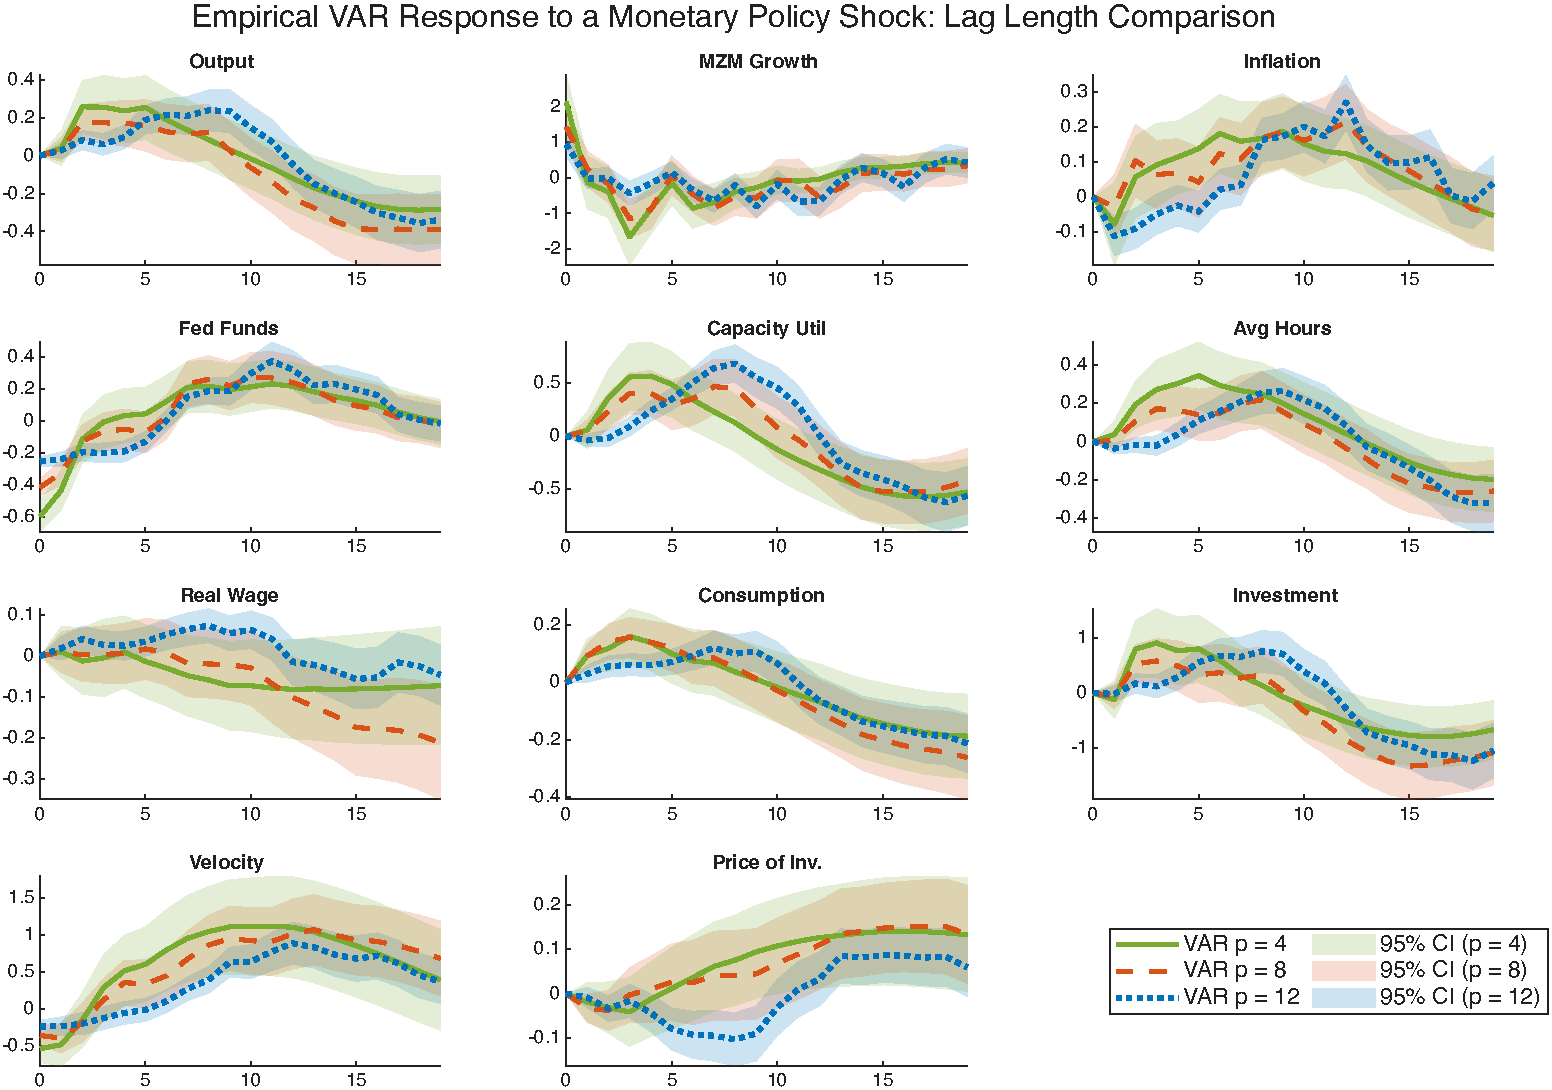
\includegraphics[width=\linewidth]{../../Output/VAR_IRFs_Long_Lag_CI_PE_4_8_12_Plots/Monetary_Policy_Shock/Comparison_Lags_4_8_12.pdf}}
    {\fbox{Image Path Broken or File Missing}}
    \caption{VAR impulse responses to a monetary policy shock across lag orders, each with its
    own $95$ percent bootstrap confidence band.}
    \label{fig:var_irfs_ci_all_lags}
\end{figure}
\FloatBarrier

The bands at $p=12$ are not wider than those at $p=4$, and for several variables they are
visibly narrower, despite the threefold increase in parametrisation. The same pattern appears
in the structural estimates, where the Phillips curve slope is estimated roughly six times more
precisely at $p=12$. The variance reduction mechanism therefore operates at the parametrisation
frontier, which is a considerably more demanding test than the two variable systems in which it
was first demonstrated.

\tbd{Quantificare invece di ``visibly narrower'': larghezza media della banda per variabile e
lag order, e rapporto medio $p=12$ contro $p=4$. Una riga di numeri.}

Two features of the construction matter for reading the figure. The bands are bootstrap bands
in which the entire VAR is re-estimated on each artificial sample, so the uncertainty induced by
estimating $1{,}210$ coefficients is propagated rather than conditioned away. Had the estimator
been unstable at $p=12$, the re-estimated responses would have varied wildly across draws and
the bands would have widened accordingly. Draws yielding an explosive companion matrix are
discarded and redrawn, so the bands condition on stationarity.

The obvious objection is that this is overfitting. A VAR with $121$ regressors per equation
fits the sample closely, the residuals shrink, and bands computed from those residuals shrink
with them. The objection has to be taken seriously, because in sample it cannot be dismissed:
reduced misspecification and overfitting share the same signature. What can be said is that the
bootstrap re-estimation rules out the mechanical part of the concern, since parameter
uncertainty is not being suppressed. What it cannot rule out is that the residual variance is
itself understated, because the bootstrap resamples from the fitted residuals of the model
under scrutiny. Distinguishing the two requires evidence that is not in sample, which is
precisely what \citet{Long_Lag2025} supply through coverage rates computed where the true
responses are known.

% =============================================================
% END BODY
% =============================================================

\clearpage
\bibliographystyle{apalike}
\bibliography{biblio_ch23}

\end{document}